\chapter{Background} \label{chap:background}

This chapter is dedicated to equipping the reader with the understanding of the properties of MongoDB that make it susceptible to durability failures and how these are addressed in the MongoDB architecture by providing them with relevant background knowledge of MongoDB and its replication mechanisms. We expand upon the \prettyref{sec:lit-mongo} focusing on the technical details relevant to our contributions. The material is taken from the online documentation, code and explanations from experts on MongoDB.

\section{MongoDB}
\label{sec:mongodb}
A MongoDB database holds \textit{collections} of \textit{documents}, where a collection is the equivalent of a table and a document is equivalent to a row in a relational database. Each document may contain an arbitrary arrangement of fields and values - not being limited by a schema.

MongoDB is able to provide high availability and redundancy via \textit{replica sets}. A MongoDB replica set is comprised of an odd number of MongoDB instances, each maintaining a copy of the same set of data. Through an automatically orchestrated election, one of these instances is determined as the \textit{primary} replica, while the remaining nodes are labeled as \textit{secondary} replicas. Only the primary replica will receive write operations propagating those writes to the secondaries via the \textit{Oplog}. The secondary replicas will continuously read and apply the changes in the Oplog on their own data set as to maintain identical data to the primary.

MongoDB's default storage engine is WiredTiger. This engine regularly creates snapshots of the data and writes them to disk in a consistent way across all data files. These snapshots are therefore durable and can act as recovery checkpoints in case of data corruption. During the writing of a new snapshot, the previous snapshot remains valid. As such, if MongoDB encounters an error while writing the snapshot, it can use the previous one to recover. By default, WiredTiger is configured to create snapshots every 60 seconds.

To complement long-term durability guarantees of snapshots, WiredTiger implements a write-ahead transaction log to persist all data modifications between checkpoints. WiredTiger creates one journal record for each client-initiated write operation and assigns it a unique identifier. This includes any internal writes that are initiated by the database as a consequence of the client operation (e.g. updating indexes). WiredTiger buffers these writes in-memory, persisting them to disk every 50 milliseconds.

\section{Replication}
\label{sec:replication}
A functioning MongoDB replica set requires that a primary node to always be up. This is because only the primary can accept write operations and propagate those writes to the secondary nodes. When a primary receives a write operation from a client, at minimum, it will perform the operation on its copy of the data before responding to the client with an acknowledgement of this operation. The primary will proceed by journaling the write and waiting for the journal to flush to disk. After the flush, the primary will add the operation into its Oplog.

The secondary replicas then read the Oplog and apply these operations to their own copy of the dataset. Once an operation is applied, the secondary sends an acknowledgement of this operation to the primary for it to track how many nodes have applied each operation to their copy of the data. This process insures that a secondary replica has data that is consistent with the primary up to a fixed point in time. As such, in the event of a failure in the primary, a secondary node can take over its role while suffering minimal data loss.

To maximise the speed of replication, each secondary has a cursor that points to the end of the primary's Oplog. When a new write operation is performed, the primary adds the operation to the Oplog and notifies the replicas that the Oplog has been updated. The replicas proceed to move their cursors forward, applying the new operations and updating their own Oplog. 

As all secondary nodes have their cursors pointing to the same Oplog, they will all process the operations in the same order. This means that at any point, all replicas will have a \textit{common} prefix of all write operations submitted to the primary node i.e. if there are two writes $w_1$ and $w_2$, it is \textit{impossible} for one replica to have \textit{only} $w_1$ and another to only have $w_2$.

\section{Failure Detection \& Election}
\label{sec:election}
In order to maximise availability, MongoDB uses a simple heartbeat scheme to automatically detect when a replica set member fails. Each node sends heartbeats (pings) to all other nodes every two seconds. If the node fails to reply to a heartbeat within a preconfigured amount of time (10 seconds by default), the replica member sending the heartbeat will mark it as inaccessible. 

If the inaccessible node is a secondary replica member, no further work is performed by the replica set, as the functioning primary can still process write operations and queries. If a primary is marked as inaccessible, the member that detected the failure will call an election to select a new primary. The elected primary is guaranteed to have the most up-to-date view of the data. That is, if secondary A saw an operation $o$ but secondary B hasn't, then secondary A will become the new primary.

\section{Write Concern}
\label{sec:writeconcern}
The \textit{write concern} setting in a MongoDB client allows each client to configure the strength of write acknowledgement independently. Upon issuing a write operation, the client is blocked until it receives an acknowledgement of the operation. Our study uses the \textit{w : 1, journaled and majority} settings of write concern.

The most permissive, and hence performant, write concern \textit{w : 1} (also referred to as primary write concern) acknowledges the write just after the primary applies the operation on its data. This value can be modified to be \textit{w: k} where the primary will wait for $k-1$ secondary replicas to acknowledge the write before the primary sends an acknowledgement to the client. An example of a w:1 execution can be seen in \prettyref{fig:writecon-primary}

The \textit{journaled} setting builds on this, delaying the acknowledgement until after the primary persists the operation into the journal. The journal does not immediately write persist the operation on disk, instead buffering multiple operations before persisting them to the journal as a batch as seen in \prettyref{fig:journal_buffer}. An example of journaled execution can be seen in \prettyref{fig:writecon-journaled}.

Finally, \textit{majority} will not acknowledge the write until more than half of the nodes have also acknowledged it. An example of this is seen in \prettyref{fig:writecon-majority}. We should bring your attention to the fact that the only change between figures \ref{fig:writecon-primary}, \ref{fig:writecon-journaled} and \ref{fig:writecon-majority} is the time at which the acknowledgement is sent back to the client.

\begin{figure}
    \centering        
    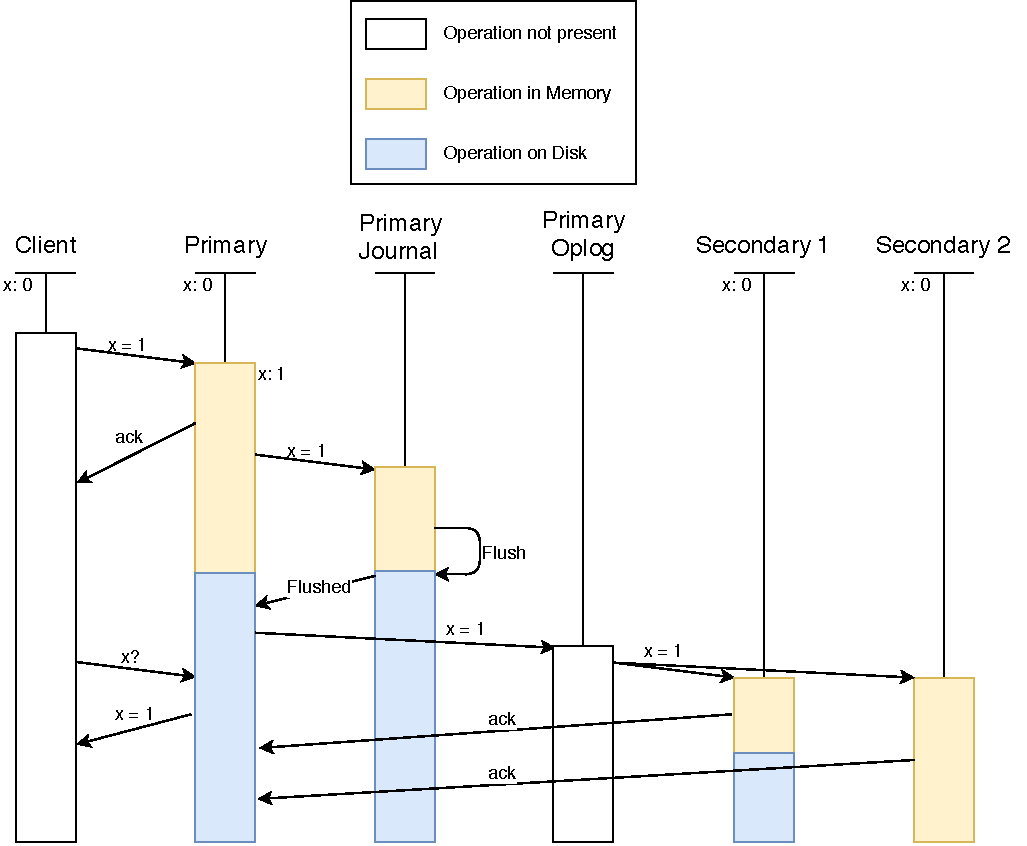
\includegraphics{images/PrimaryWriteConcern.pdf}
    \caption{Time-space diagram of how a write operation behaves with \textit{primary} write concern}
    \label{fig:writecon-primary}
\end{figure}

\begin{figure}
    \centering
    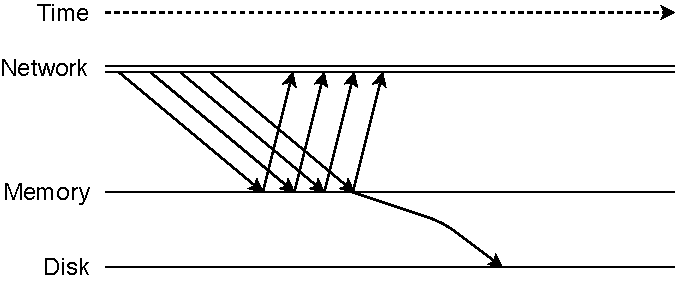
\includegraphics[width=\textwidth]{images/Buffering.pdf}
    \caption{Time-space diagram of MongoDB buffering writes from the network before journaling.}
    \label{fig:journal_buffer}
\end{figure}

\begin{figure}
    \centering        
    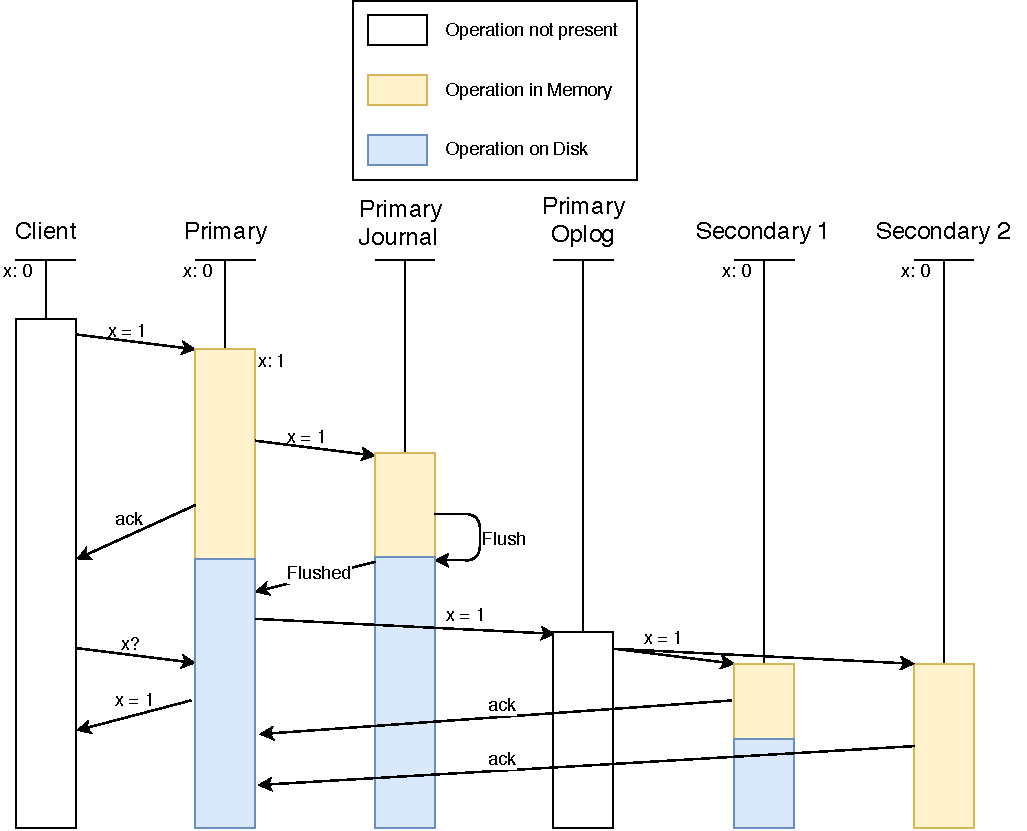
\includegraphics{images/JournaledWriteConcern.pdf}
    \caption{Time-space diagram of how a write operation behaves with \textit{journaled} write concern.}
    \label{fig:writecon-journaled}
\end{figure}

\begin{figure}
    \centering        
    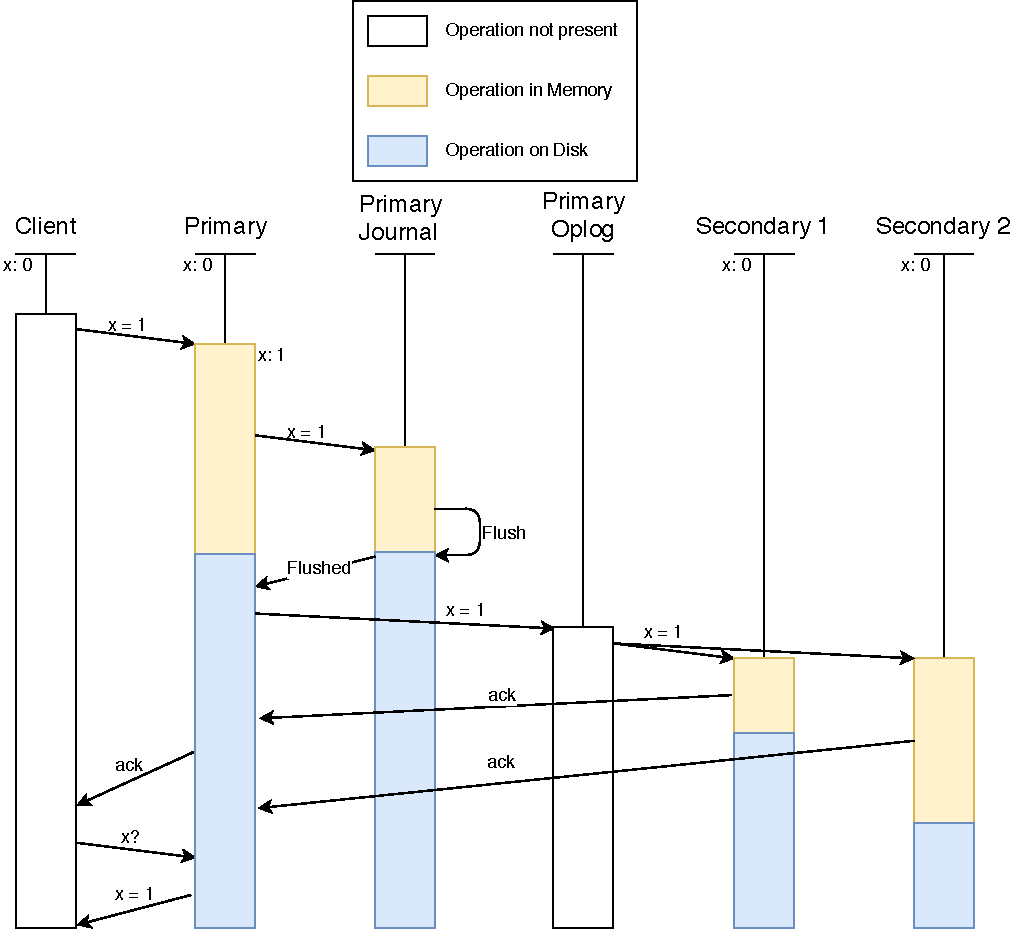
\includegraphics{images/MajorityWriteConcern.pdf}
    \caption{Time-space diagram of how a write operation behaves with \textit{majority} write concern.}
    \label{fig:writecon-majority}
\end{figure}

\section{Read Concern}
The MongoDB \textit{read concern} option allows each client to control the consistency properties of the data read from a replica set. Our study uses the \textit{local, majority and linearizable} settings for the read concern.

Clients making a query with a \textit{local} read concern will retrieve the most recent data from the replica that received the read request. A query with \textit{majority} read concern will return data that has been acknowledged by a majority of the replica set members, while \textit{linearizable} concern will return data that reflects all majority-acknowledged writes completed prior to the start of the query.

\section{Read Preference} \label{sec:readpref}

The \textit{read preference} setting specifies how a client will route queries to the MongoDB replica set. By default, all reads are sent to the primary, however this can be changed to increase availability. Our experiments use the \textit{primary, primary preferred and secondary} settings.

The \textit{primary} setting is the default and will only query the primary replica for data. The \textit{primary preferred} setting is effectively the same as default, but uses secondary replicas as a fallback if the primary appears to be down. The \textit{secondary} preference will never query the primary replica.

\section{MongoDB vs Dynamo}
In the previous chapter, we discussed MongoDB and Dynamo as two types of NoSQL databases, with MongoDB acting as a document store, while Dynamo being a simpler key-value store. We now bring your attention to the differences in the way these two systems perform replication and sustain high availability.

While MongoDB uses a Primary-Secondary replication scheme and requires the primary to first acknowledge an operation before propagating it to the secondaries, Dynamo utilises a multi-master scheme. In Dynamo's scheme, every replica is in charge of a chunk of the total data and every replica can accept a write operation. Upon receiving a write operation, a Dynamo replica will apply the operation to its copy of the data if the key is in its range, and forward the operation to other nodes in charge of this data item. This way, Dynamo ensures high availability of its data and failure tolerance. 

We should also note that MongoDB's Primary-Secondary replication scheme requires an election if the Primary fails. An election can potentially reduce the availability of the system, as no write operations can be accepted while a Primary is unavailable. On the other hand, Dynamo's multi-master strategy utilises a gossip-based protocol for identifying failed replicas, which allows it to stay completely available while replicas rearrange themselves to spread out the load and data of the failed replica, using replication as the means of ensuring durability.

While Dynamo's properties have been extensively researched, the fundamental differences between the designs of these two systems warrant a in-depth look into MongoDB.